\documentclass{beamer}
\mode<presentation>
\usetheme{CambridgeUS}
\usepackage[russian]{babel}
\usepackage[utf8]{inputenc}
\usepackage[T2A]{fontenc}
\usepackage{sansmathaccent}

\usepackage{verbatim}
\usepackage{alltt}

\pdfmapfile{+sansmathaccent.map}
\title[Color patterns]{Цветовое прототипирование}
\author{Наумов Д.А., доц. каф. КТ}
\date[29.02.2020] {Базы данных и базы знаний, 2020}

\begin{document}

\begin{frame}
  \titlepage
\end{frame}
  
\begin{frame}
  \frametitle{Содержание лекции}
  \tableofcontents  
\end{frame}
  
\section{Прототипирование}
\subsection{Концептуальные классы}
\begin{frame}
\begin{block}{Модель предметной области}
визуальное представление концептуальных классов или объектов реального мира в терминах предметной области.
\end{block}
\begin{block}{Концептуальный класс}
описание совокупности объектов с общими атрибутами, операциями и семантикой.
\end{block}
Категории концептуальных классов:
\begin{itemize}
\item физические и материальные объекты;
\item спецификации, каталоги, правила, руководства;
\item места, контейнеры объектов и содержимое контейнеров;
\item транзакции и элементы транзакций;
\item организации; 
\item процессы и события, записи деятельности;
\item роли людей или предметов;
\item абстрактные понятия.
\end{itemize}
\end{frame}

\begin{frame}
\begin{block}{Связь}
описание некоторого смысловое отношения между обьъектами.
\end{block}
Категории отношений:
\begin{itemize}
\item объект А является физической/логической частью объекта B;
\item объект А является элементом отчета объекта B;
\item объект А является организациюонной единицей объекта B;
\item объект А использует/взаимодействует с объектом B;
\item объект А следует за объектом B;
\item объект А является событием, связанным с объектом B.
\end{itemize}
\end{frame}

\subsection{Прототипы}
\begin{frame}
\begin{block}{Прототип}
способ классификации объектов предметной области по признакам, которым они более или менее соответствуют.
\end{block}
\begin{itemize}
\item в процессе анализа и построения моделей предметных областей были выделены и каталогизированы шаблоны, позволяющие ускорить процесс моделирования [Coad, North, Mayeld, 1997];
\item одним из предложенных механизмов был механизм цветового прототипирования;
\item модели предметной области часто создают путем мозгового штурма, наклеивая цветные бумажки на доску.
\end{itemize}
Виды прототипов:
\begin{itemize}
\item момент или интервал (розовый)
\item роль (желтый)
\item группа, местоположение или предмет (зеленый)
\item описание (голубой)
\end{itemize}
Объекты, относящиеся к одному прототипу, имеют прогнозируемые отношения с другими объектами.
\end{frame}

\begin{frame}
\begin{block}{Описание (голубой)}
обозначение типа предметов. 
\end{block}
Пример:
\begin{itemize}
\item тип книги;
\item жанр фильма;
\item модель автомобиля;
\item элементы каталога (ОКЕИ, ОКАТО, ОКВЭД и т.п.).
\end{itemize}
\begin{center}
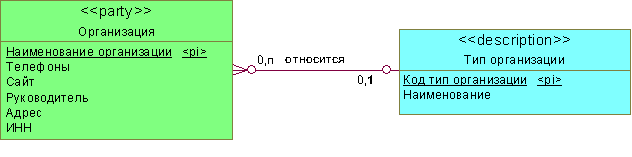
\includegraphics[scale=0.5]{images/lec03-pic05.png}
\end{center}
\end{frame}

\begin{frame}
\begin{block}{Группа объектов (зеленый)}
используются для обозначения групп, местоположения или предметов. 
\end{block}
Пример:
\begin{itemize}
\item книги;
\item фильмы;
\item сотрудники;
\item предметы;
\item организации.
\end{itemize}
\begin{center}
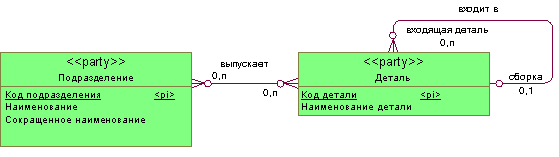
\includegraphics[scale=0.7]{images/lec03-pic03.png}
\end{center}
\end{frame}

\begin{frame}
\begin{block}{Момент-интервал}
самые динамичные объекты, связанные с моментом или интервалом времени.
\end{block}
Пример:
\begin{itemize}
\item продажа;
\item счет-фактура;
\item резервирование;
\item планы полетов;
\item аренда;
\item оплата и т.д.
\end{itemize}
\begin{center}
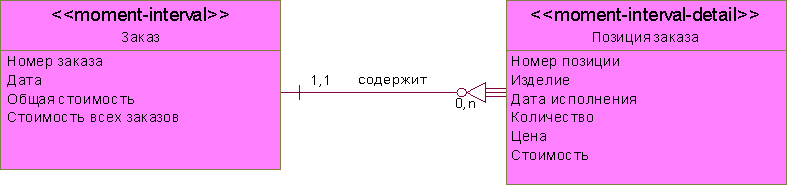
\includegraphics[scale=0.5]{images/lec03-pic02.png}
\end{center}
\end{frame}

\begin{frame}
\begin{block}{Роль (желтый)}
обозначения ролей, которые выполняют объекты, участвуя в действии в "розовые" моменты времени.
\end{block}
Пример:
\begin{itemize}
\item должность;
\item место хранения;
\end{itemize}
Обычно роли выполняются людьми, иногда  местами расположения или предметами.
\begin{center}

\includegraphics[scale=0.45]{images/lec03-pic04.png}
\end{center}
\end{frame}

\begin{frame}
Зеленые объекты играют желтые роли при участии в действиях в розовые моменты времени и описываются голубыми описаниями.
\begin{itemize}
\item Книгу можно отдать во временной пользование (желтая роль).
\item Автомобиль (зеленый предмет) может быть продан (желтая роль) в процессе продажи (розовый интервал).
\end{itemize}
\begin{center}
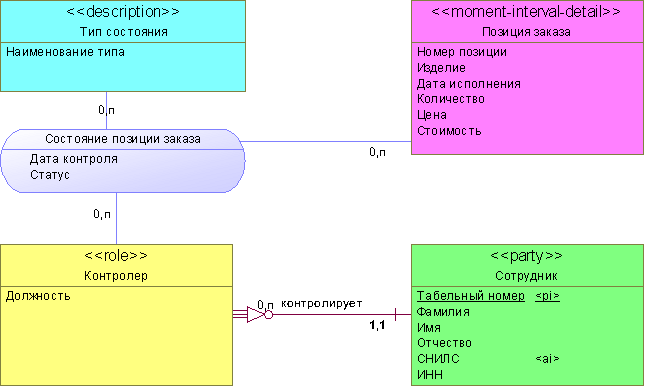
\includegraphics[scale=0.45]{images/lec03-pic06.png}
\end{center}
\end{frame}

\begin{frame}
\begin{center}
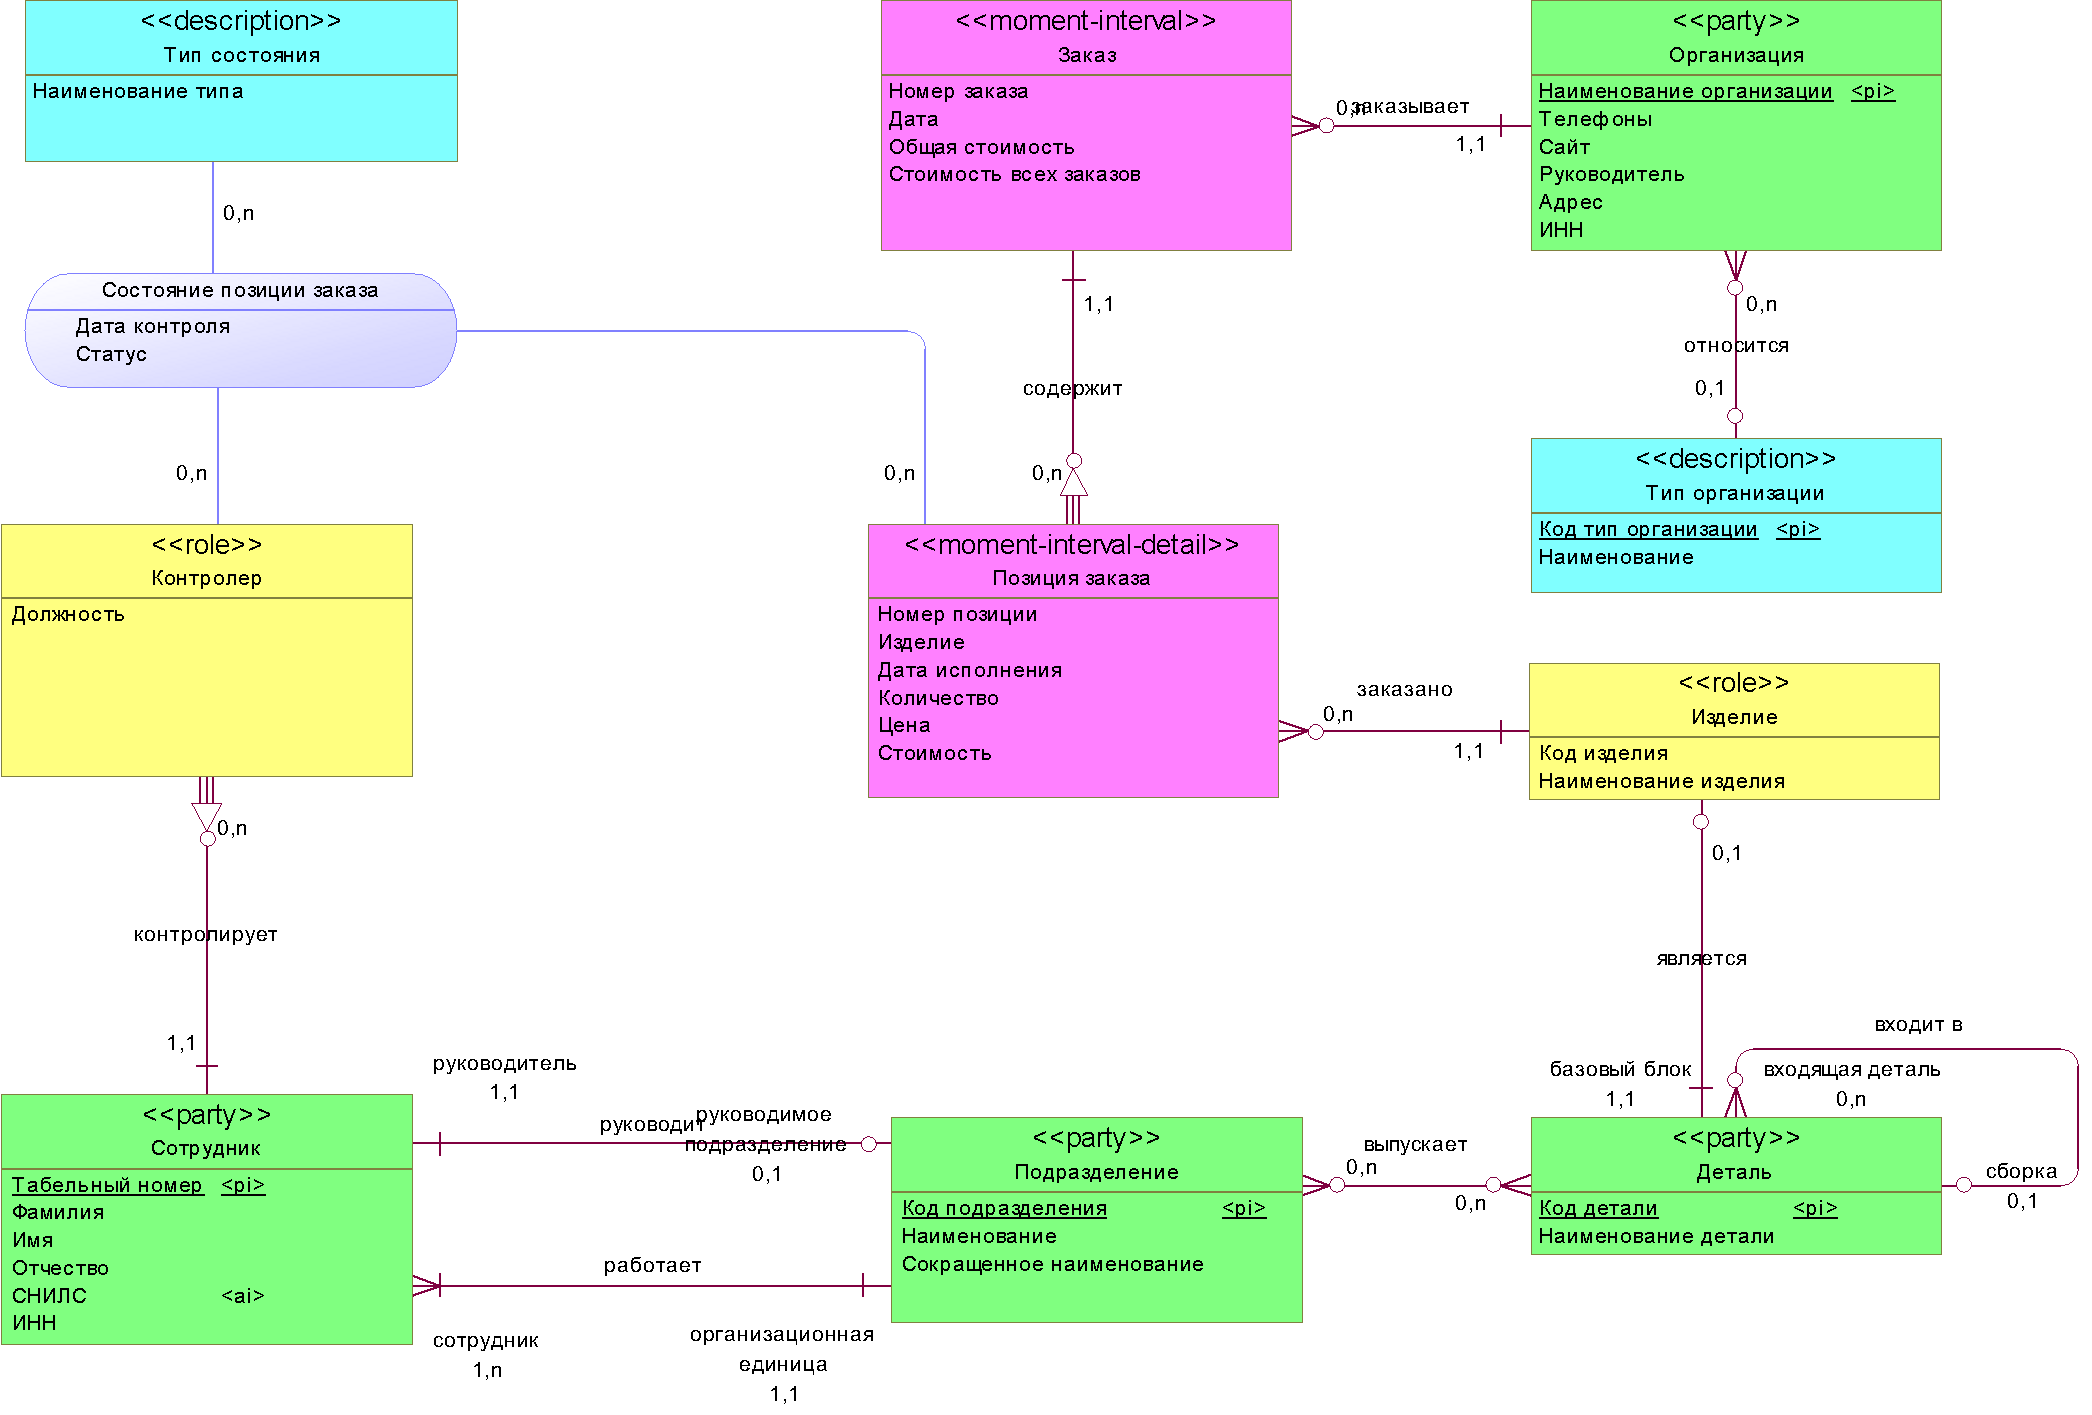
\includegraphics[scale=0.22]{images/lec03-pic01.png}
\end{center}
\end{frame}

\end{document}
